\documentclass{article}
\usepackage[utf8]{inputenc}
\usepackage{amssymb, amsmath,hyperref,verbatim,listings,graphicx,subfigure,fullpage}

\begin{document}

\title{UML computer project 1}
\author{
Juha-Antti Isojärvi\\
013455341 \\
Department of Mathematics and Statistics\\
Master student
\and
Mikko Sysikaski\\
013573016\\
Department of Computer Science\\
Master student}
\date{}
\maketitle

\section{Exercise set 1}
\subsection{Exercise 1}
First we were given plots of twodimensional data, and were asked to
create similar data artificially. The distribution of the data in the plots looked
similar to the twodimensional gaussian or multinormal
distributions. Therefore we decided to generate points from a
gaussian distribution. 

A random vector $X = (X_1, X_2, \dots, X_n)$ is standard normally
distributed, denoted $X \sim N_n(0,I)$, if its components $X_i$ are independent and normally
distributed with zero mean and unit variance. It is true, that the
mean vector $E(X) = 0$ and covariance matrix $Cov(X) = I_n$.

Now if a random vector 
\[
X = AU + \mu
\] 
is defined for some $U \sim N_n(0,I)$, and fixed $A \in \mathbb{R}^{m \times n}$
and $\mu \in \mathbb{R}^n$, then it is true that $E(X) = \mu$ and
$Cov(X) = AA^T$.

A random vector $X$ is multinormally
distributed, if it has the same
distribution as the random vector
\[
X = AU + \mu.
\]
Then it has mean $E(X) = \mu$ and covariance $Cov(X) = AA^T$. Denote
$Cov(X) \dot{=} \Sigma$. The multinormal distribution is denoted $X
\sim N_n(\mu,\Sigma)$.

It also holds, that if $X \sim N_n(\mu,\Sigma)$, and $B \in
\mathbb{R}^{m \times n}$ and $b \in \mathbb{R}^m$ are fixed, then 
\[
BX + b \sim N_m(B\mu + b, B \Sigma B^T).
\]

Now, one way of simulating gaussian twodimensional data, is to first
simulate twodimensional standard normally distributed, i.e. white, data, and then
affinely transform this data by multiplying with some matrix $A \in
\mathbb{R}^{2\times 2}$. The affinely transformed data has then a
gaussian distribution with zero mean and covariance $AA^T$.

So, we generated two random samples from a normal distribution and put these
together to form twodimensional white data. If one would plot this
data, one would see a spherical point cloud centered at zero. Then we
dilated this cloud in the $y$- and $x$-axis direction with multiplying by a dilation matrix $D$ and then rotated
the dilated data cloud with multiplying by a rotation matrix
$R_\theta$. The result was a sample from the 
distribution $N_2(0,AA^T)$, where $A \dot{=} R_\theta D$.

The resulting data cloud is centered at zero, and has elliptical
shape. The main axis of this data cloud has angle $\theta$ measured
form the $x$-axis. The spread of the cloud is determined by the
dilation matrix $D$. Our resulting four generated artificial data can be
seen plotted in Figure~\ref{fig:scatter}. 

This was a simple method for generating artificial twodimensional
gaussian data, with easy control of the direction and elongation of
the data cloud. Of course there are other methods as well. In the
MASS-package of R there is a function rmvnorm, which takes as
inputs the mean vector and the covariance matrix and generates
gaussian data. We
didn't feel the need to get further into the details of this
method. Manipulation of the direction and the elongation of the data
cloud is always achieved by manipulation of the covariance matrix, as
in the method we described.

Another way of manipulating the direction and elongation of the data
cloud is by 'inverse' eigenvalue decomposition of the covariance
matrix. About this method more in section \ref{sec:subsection4}.

\newcommand{\sscale}{0.5}
\begin{figure}\centering
	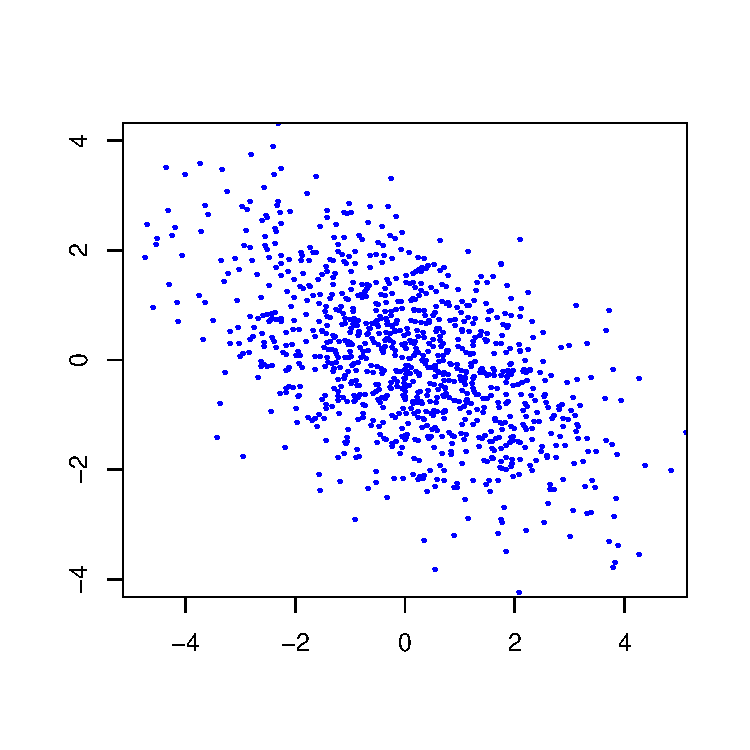
\includegraphics[scale=\sscale]{scatter1}
	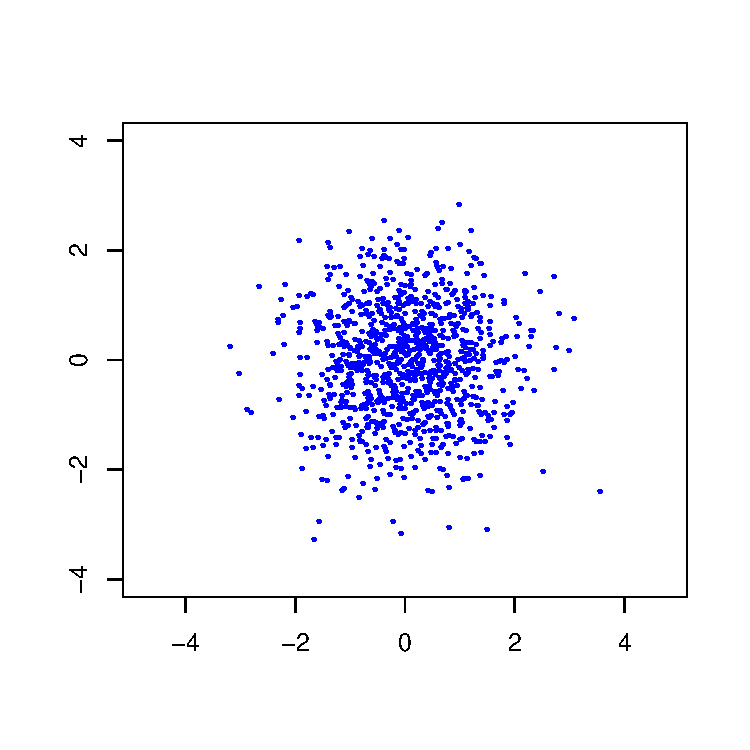
\includegraphics[scale=\sscale]{scatter2}

	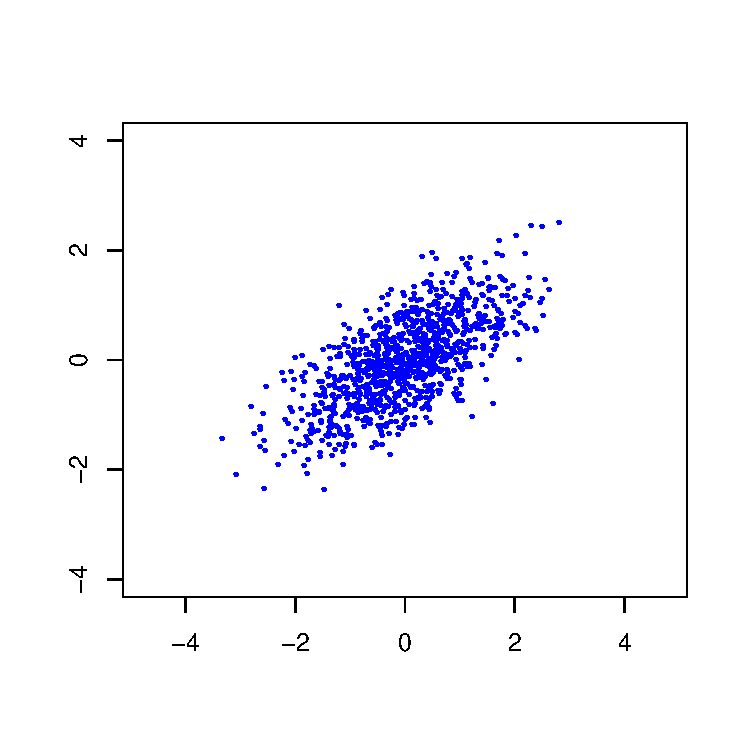
\includegraphics[scale=\sscale]{scatter3}
	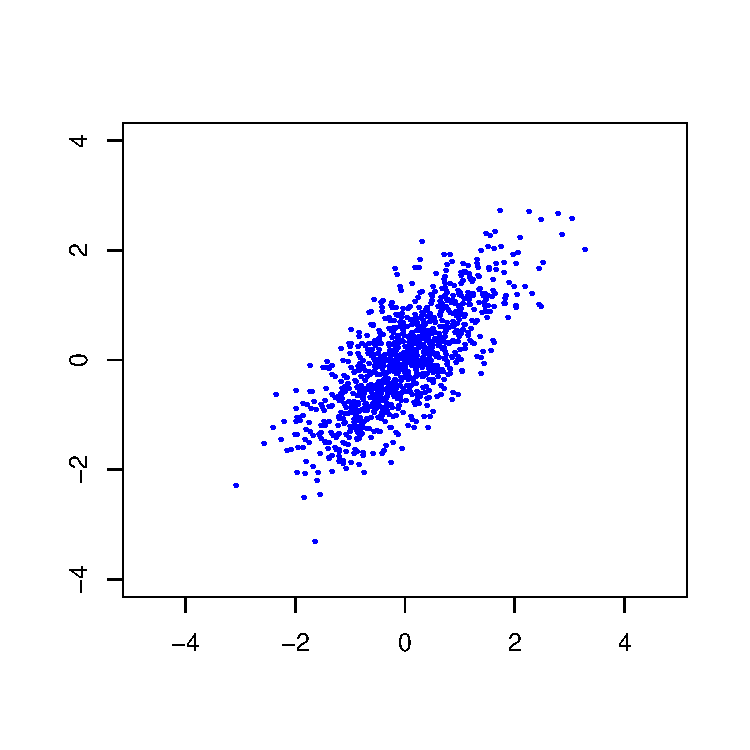
\includegraphics[scale=\sscale]{scatter4}
	\caption{The scatter plots of the data generated in task 1.1.} \label{fig:scatter}
\end{figure}

\subsection{Exercise 2}

Next, we were given the task to perform principal component analysis
on two of the generated artificial data. We chose the data seen in
Figure \ref{fig:scatter} in the upper left and lower left frame.

In order to do principal component analysis, we first need the
covariance matrix of the data. In the context of PCA one doesn't have
prior knowledge of the underlying distribution, and therefore we used
the standard method of computing a sample covariance matrix. In R this
can be done with the function cov. 

Next we did eigenvalue decomposition of the covariance matrix. In the
lecture notes it is proven that the first principal component is the
eigenvector corresponding to the largest eigenvalue, the second PC the
eigenvector corresponding to the second largest eigenvector, and so
on. In this case of twodimensional data there are only two principal
components. The directions of the principal components of the point
sets are shown in Figure~\ref{fig:pcadir}. 

\begin{figure} \centering
	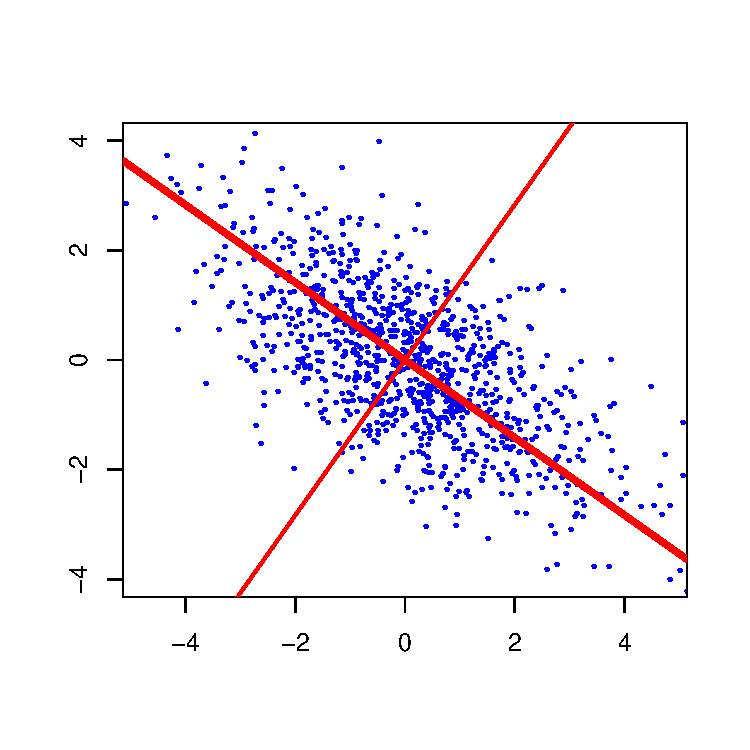
\includegraphics[scale=\sscale]{pcadir1}
	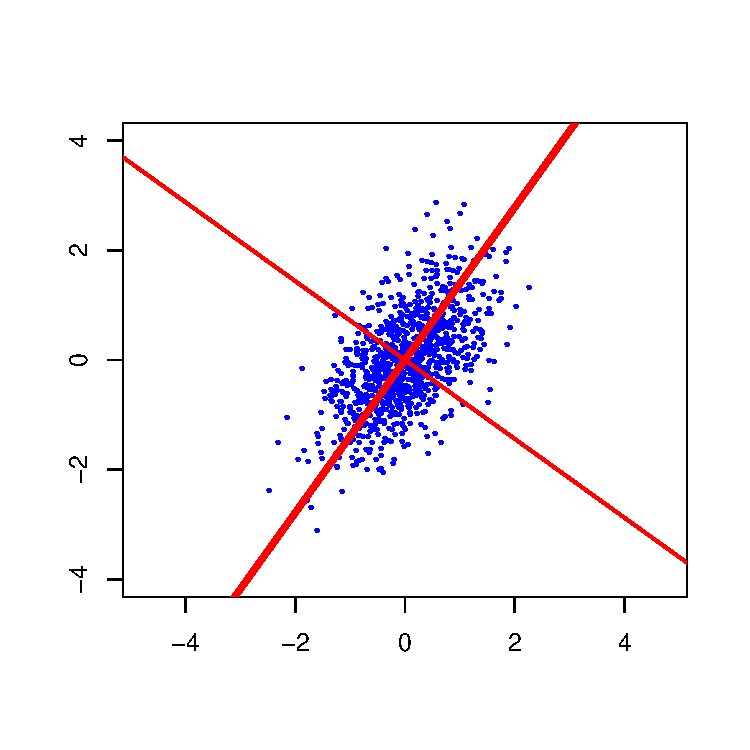
\includegraphics[scale=\sscale]{pcadir3}
	\caption{Principal components of the first and the third point set. The first PC is the bolder line.} \label{fig:pcadir}
\end{figure}

\subsection{Exercise 3}
In the third exercise of this set, we projected the first artificial data
set on each of its principal components. The projection can be done simply
by taking the dot product of each point with the principal component. Histograms of the
projected data can be seen in Figure~\ref{fig:histo}. The variance of
the projected data should be equal to the eigenvalue of the
corresponding eigenvector of the covariance matrix of the original
data. This was verified after computing the variance of the projected
data and the eigenvalue decomposition of the covariance matrix:
\begin{verbatim}
> var
[1] 2.873594 1.013940
> eig$values
[1] 2.873594 1.013940
\end{verbatim}
\begin{figure} \centering
	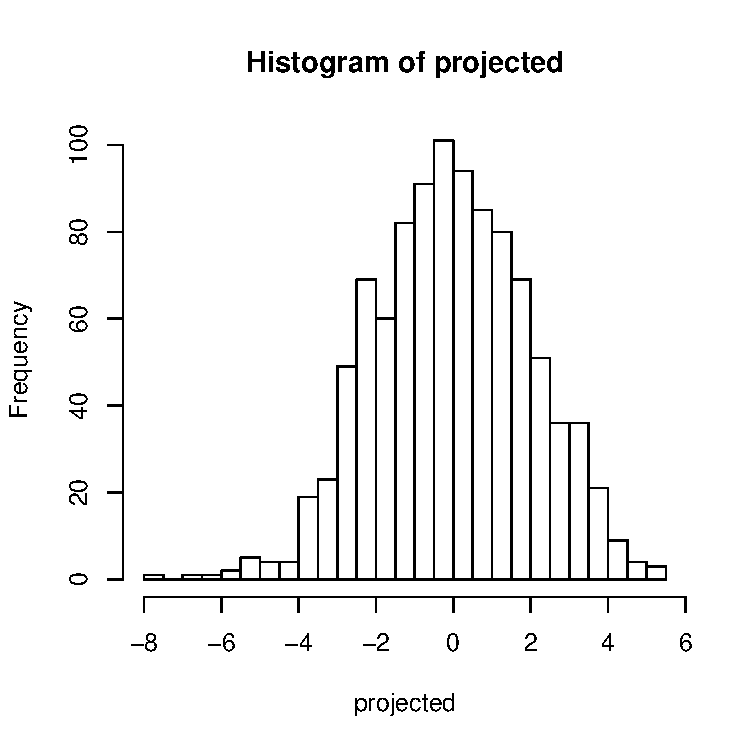
\includegraphics[scale=\sscale]{histo1-1}
	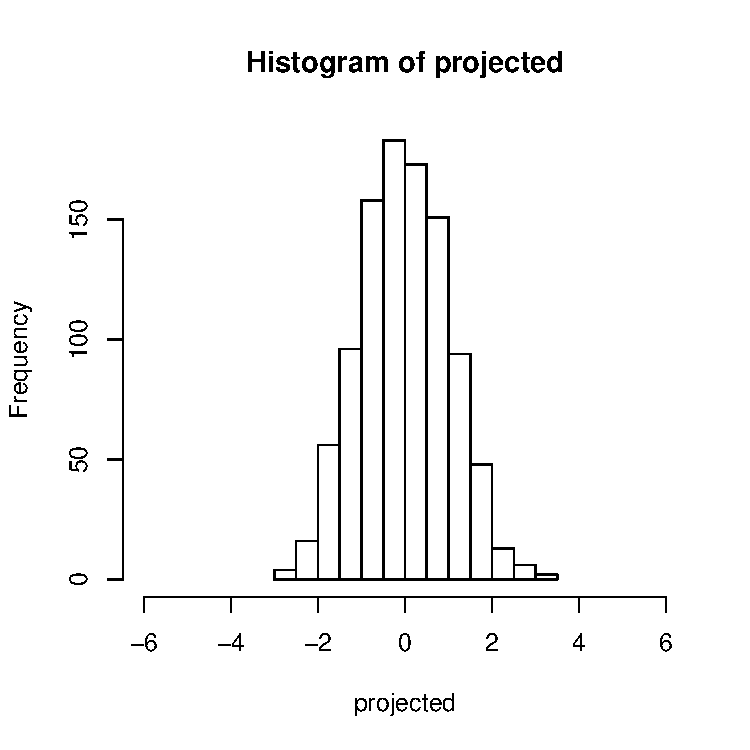
\includegraphics[scale=\sscale]{histo1-2}
	\caption{Histograms of the 1-dimensional data obtained by projecting the points of the first point set on its principal components. There is more variance in the left histogram because the first PC explains a greater proportion of the variance than the second one.} \label{fig:histo}
\end{figure}

\subsection{Exercise 4}\label{sec:subsection4}
Our next task was again to create a sample of twodimensional
artificial data. This time the principal components of the data should
be the vectors 
\[
v_1 = \frac{1}{\sqrt{2}} [1 \; 1]^T \quad \textup{ and } \quad  v_2 = \frac{1}{\sqrt{2}} [-1 \; 1]^T,
\]
and their variances should be $1$ and $3$ respectively. Because the
principal components are the eigenvectors of the covariance matrix of
the data, and their variances are the eigenvalues of the covariance
matrix, we could simply specify a symmetric, positive definite matrix 
\[
\Sigma = V \Lambda V^T,
\]
where $V = [v_1 \; v_2]$ and $\Lambda = \textup{diag}(1,3)$, and use
this matrix as the covariance input of rmvnorm of MASS in R\footnote{Note, that
one could have used, for example, Cholemskys decomposition to get 
a matrix $A$ such that $\Sigma = AA^T$, and again generate a white
sample and multiply it with $A$ to get the same result, as with rmvnorm.}. The
result can be seen in Figure~\ref{fig:vscatter}. 

The covariance matrix of the generated data is
$\left(\begin{smallmatrix}
	2.013414 & -0.927215\\
	-0.927215 & 1.874120
\end{smallmatrix}\right)$. The eigenvectors of the covariance are the principal components, so as expected, they are close to $v_1$ and $v_2$ (expect sign-reversed in case of $v_1$), and their corresponding eigenvalues are close to the specified variances 3 and 1.
\begin{verbatim}
> eigen(cov(data))
$values
[1] 2.873594 1.013940

$vectors
           [,1]       [,2]
[1,] -0.7331108 -0.6801092
[2,]  0.6801092 -0.7331108
\end{verbatim}

\subsection{Exercise 5}
Now that a sample was created we were asked to do dimension reduction
of the data so that the reconstruction error is minimized. The
dimension of the data was 2, so we could reduce the dimension only by
one. The reconstruction error of the data is minimized by doing PCA
and then reducing the dimension by projecting the data on the line
spanned by the principal component.
The 1-dimensional values can then be projected back two 2 dimensions by multiplying each of them with the same vector that was used in the projection.
In Figure~\ref{fig:proj} the first 50 points of both dimension reduced
and unchanged data can be seen plotted as well as the correspondence
between the points.

The average reconstruction error is defined as
$$ Err = E\left[\left||X-X_{red}|\right|^2\right]$$
where $X_{red}$ is the result of doing dimension reduction and projecting the result back to the original space.
The average of the reconstruction error using the first principal component was
$1.01$, and the proportion of variance explained by the first PC was $63 \%$.
Roughtly speaking, the average reconstruction error correlates with the amount of variance not explained by the components used in projection.
In more detail, the average reconstruction error should be roughly the variance of the
first principal component divided by the proportion of variance of the
first principal component explained times the proportion of variance
explained subtracted from $100 \%$.
\begin{figure} \centering
	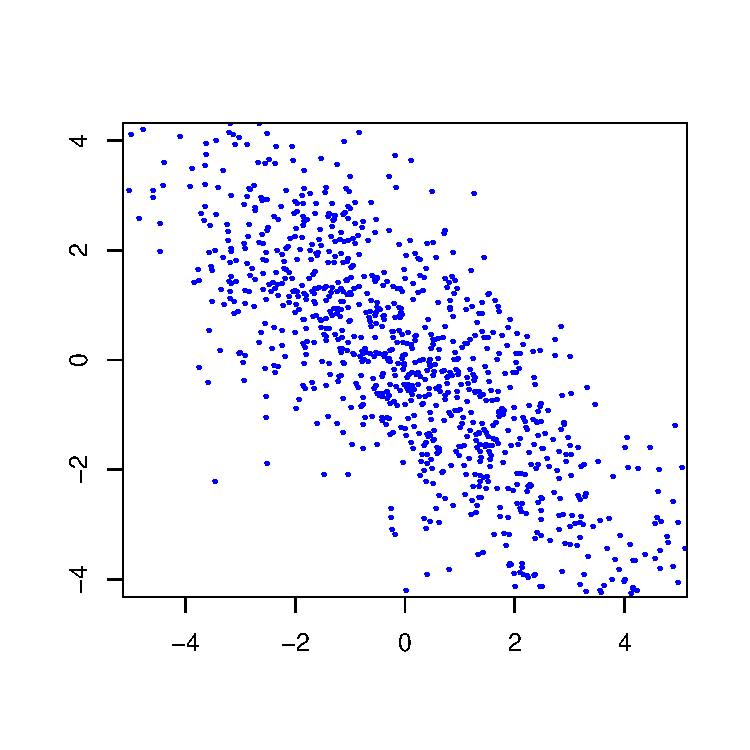
\includegraphics[scale=0.7]{vscatter}
	\caption{Scatter plot of the data generated in task 1.4.} \label{fig:vscatter}
\end{figure}
\begin{figure} \centering
	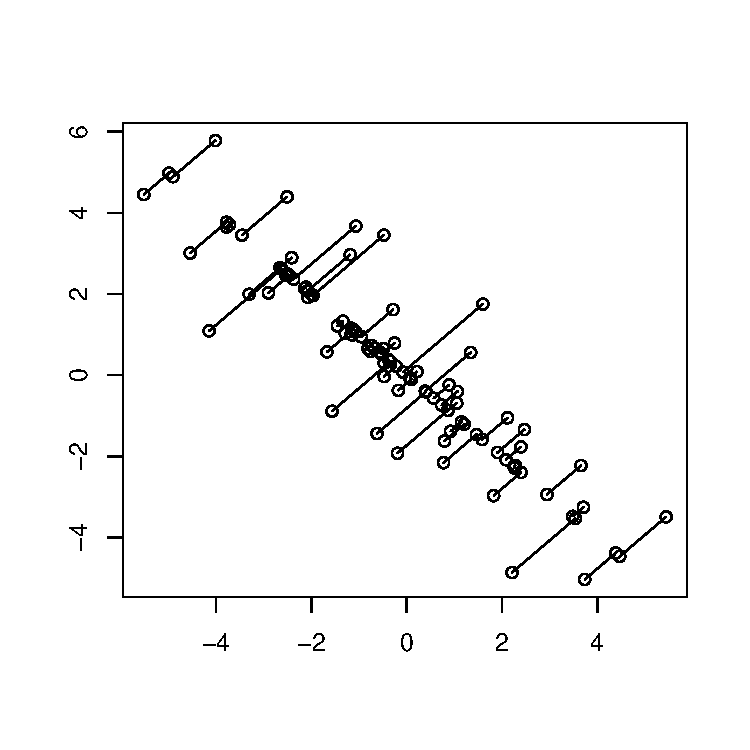
\includegraphics[scale=0.7]{proj}
	\caption{Projections of the first 50 points of Fig.~\ref{fig:vscatter} to the first principal component of the data. The original points are shown in blue and their projections in red.} \label{fig:proj}
\end{figure}


\clearpage
\section{Exercise set 2}
\newcommand{\X}{\ensuremath{\mathbf{X}}}
\subsection{Exercise 1}
The task was to do primary component analysis on the matrix
$$ X =
\begin{pmatrix}
	5 & 3 & 0 & 1 & -1 & -3 & 5 & 0 & -4 & -4 \\
	-2 & -1 & 0 & 0 & 1 & 4 & -3 & 1 & 5 & 3 \\
	0 & 1 & 4 & -1 & 0 & 5 & 5 & -5 & -3 & -3 \\
	0 & 2 & 3 & 0 & -1 & 3 & 3 & -7 & -2 & 0 \\
	3 & 4 & -2 & 1 & 3 & -3 & -3 & 2 & 0 & 0
\end{pmatrix}.
$$

The Figure~\ref{fig:42} displays the data and the original variables projected to the first two principal components.
The red lines in the figure are the projections of the original coordinate axis directions.
The length of each red line tells how much of the component is described by the first two PCs.
In other words, a short segment is an implication that the original component is relatively orthogonal to the principal components and quite a lot of the variance in its direction is lost in the projection.

\begin{figure}\centering
	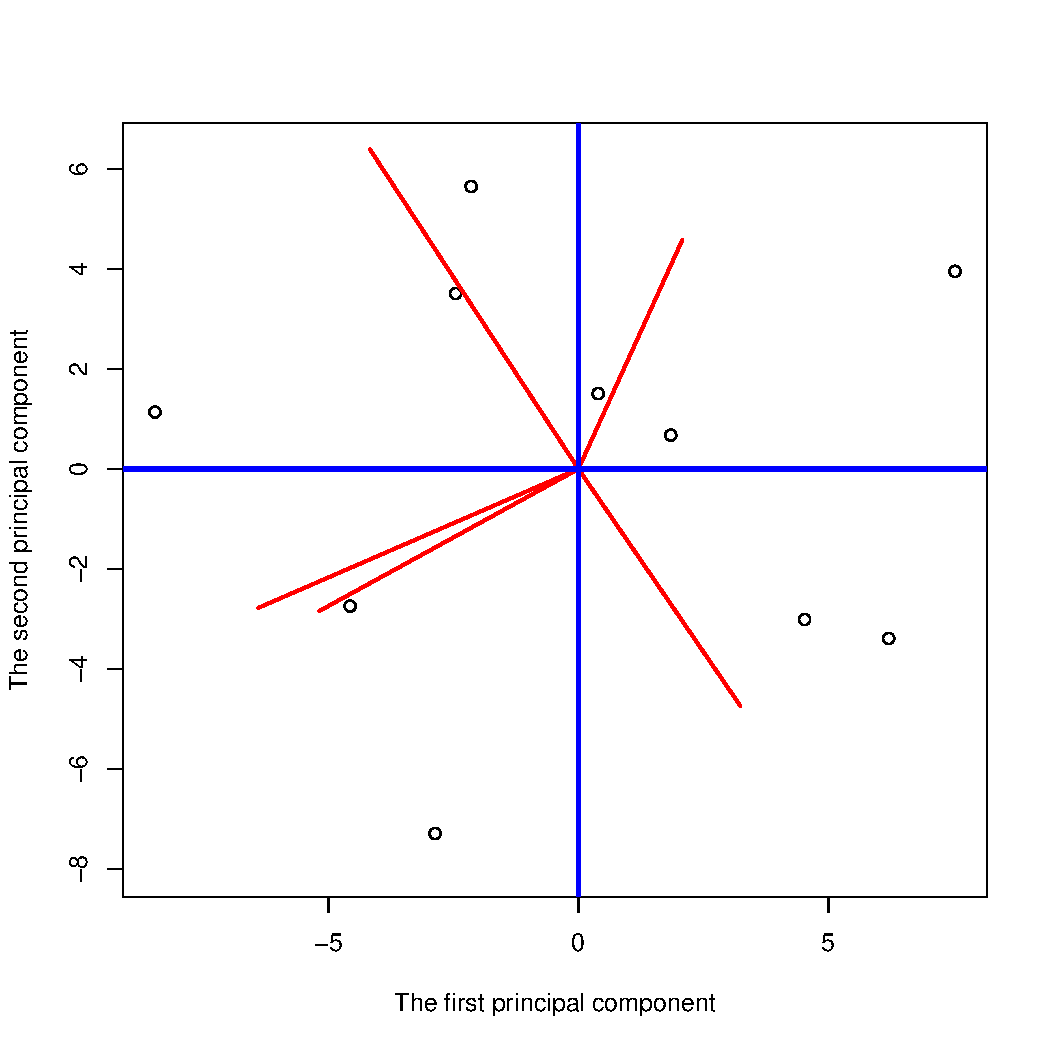
\includegraphics[scale=\sscale]{fig42}
	\caption{Reproduction of Figure~4.2 on the lecture notes.
	The blue points are the data points projected to the first two principal components.
The red lines are the projections of the original coordinate axes.}\label{fig:42}
\end{figure}

\subsection{Exercise 2}
The eigenvalues $\lambda_i$ of the covariance matrix can be interpreted as the proportions of variance explained by each principal component.
Thus the total amount of variance explained by the first $k$ principal components is equal to $$ \frac{\sum_{i=1}^k\lambda_i}{\sum_{i=1}^n\lambda_i}. $$

The amount of variance explained as a function of the number of principal components is displayed in Figure~\ref{fig:varamount}.
It can be seen that the projection to the first two components in Figure~\ref{fig:42} convey about 90.6\% of the data.

\begin{figure}\centering
	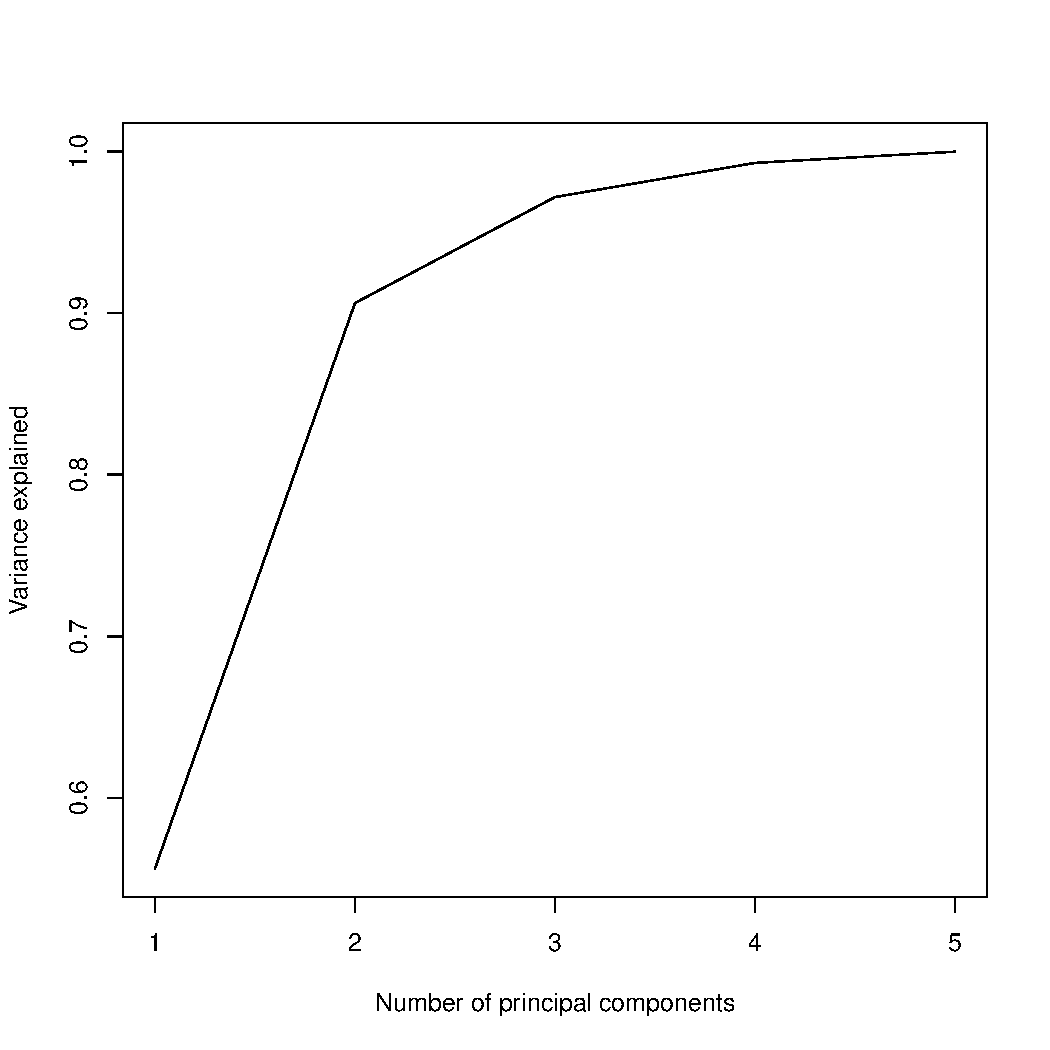
\includegraphics[scale=\sscale]{varamount}
	\caption{The proprotion of the variance explained by using only some of the principal components.}\label{fig:varamount}
\end{figure}

\subsection{Exercise 3}
In factor analysis we typically want to describe the data using components such that the projections of the original variables to the components contain mostly (approximately) zero values, as that makes the new components easier to interpret.
The quartimax rule is one way to archieve this goal.
The idea is to rotate the given components such that they span the same subspace as the original ones and maximize the sum of of fourth powers of the values of the components.
This causes many of the components to get lined with some of the original variables, and as a result the loadings of the other variables become mostly zero.

More formally, given a matrix $A$, we want to find a orthogonal matrix $U$ that maximizes
$$ J(U) = \sum_{ij}((AU)_{ij})^4. $$

We solve the problem iteratively by changing $U$ towards the gradient of $J(U)$. The partial derivative of $J$ is
$$ \frac{\partial J(U)}{\partial U_{ab}} = \sum_i4A_{ia}((AU)_{ib})^3$$
and thus the gradient if $\nabla J(U)=4A^T(AU)^3$.

As the change may make $U$ non-orthogonal, we orthogonalize the result by the formula $(UU^T)^{-1/2}U$.

To find the quartimax rotation, we thus simple start from identity matrix, and iteratively move towards the gradient and orthogonalize the result until the search converges.

When applied to the matrix
$$ A =
\begin{pmatrix}
	-0.9511 & 0.9511 \\
	-1.6435 & -1.6435 \\
	 2.3655 & 2.3655 \\
	-2.9154 & -2.9154 \\
	-3.7010 & 3.7010
\end{pmatrix}$$
we get the result
$$ U =
\begin{pmatrix}
	0.7071 & 0.7071\\
   -0.7071 & 0.7071
\end{pmatrix} $$
and
$$ A^* = AU =
\begin{pmatrix}
	0 & -1.3450 \\
	-2.3243 & 0\\
	 3.3453 & 0\\
	-4.1230 & 0\\
		  0 & -5.2340
\end{pmatrix} $$
which is identical to the example in the lecture notes, except that the values in the second column are negated.

\subsection{Exercise 4}
We applied the quartimax to the first two principal components of \X, and multiplied the components by the resulting orthogonal matrix. The result of projecting the columns of \X\ to the rotated components is displayed in Figure~\ref{fig:qmax}.
The figure is identical to the Figure~\ref{fig:42}, only the axes are rotated.
This highlights the fact that the rotation doesn't change the subspace spanned by the principal components, so they explain the same variance before and after the rotation.

\begin{figure}\centering
	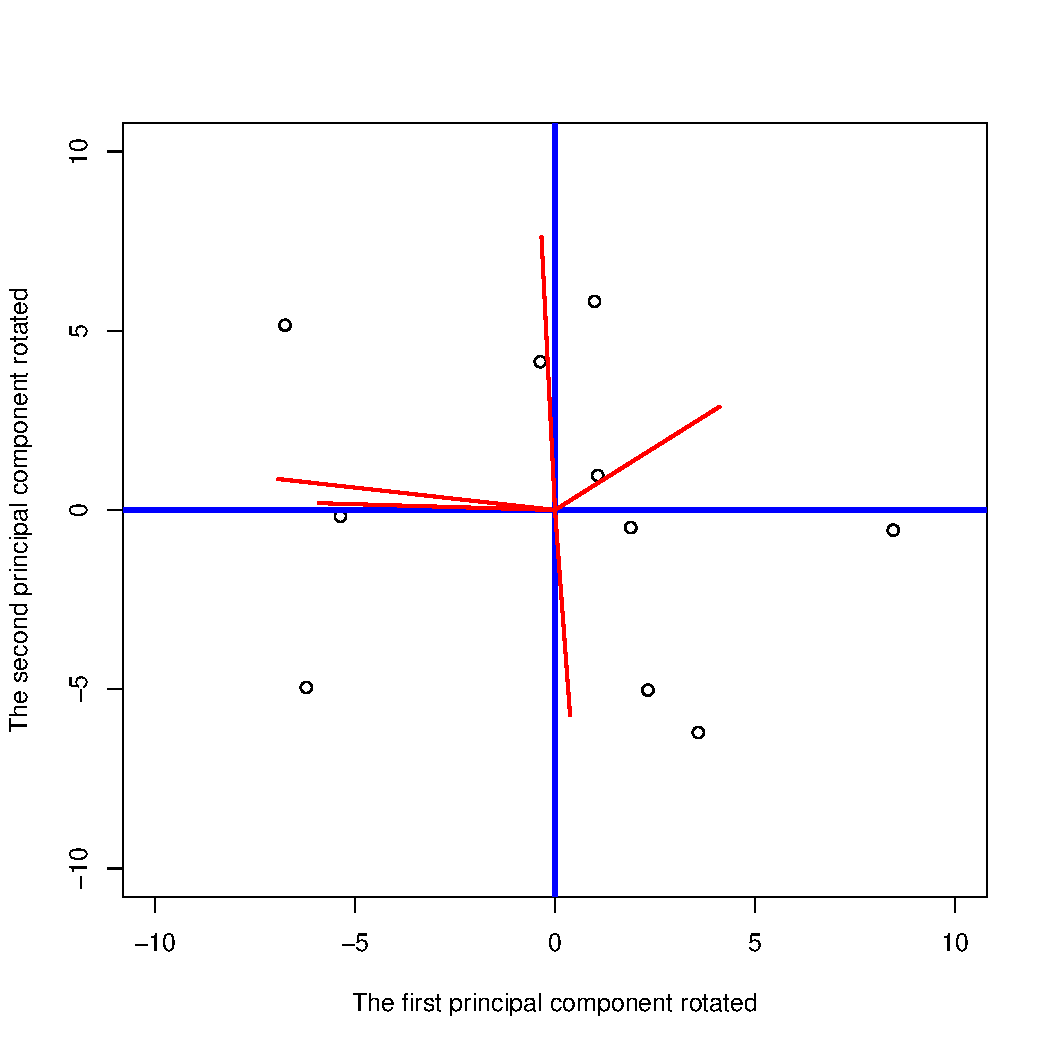
\includegraphics[scale=\sscale]{qmax}
	\caption{The projection to principal components after rotating them using the quartimax algorithm to have the original variables as close to the new coordinate axes as possible.}\label{fig:qmax}
\end{figure}


\clearpage
\section{Exercise set 3}
\subsection{Exercise 1}\label{sec:31}
The data was preprocessed by first looking at each digit separately.
For each digit we removed the average of the values and normalized then to unit norm.
Finally we again took all the images together and centered each variable to have mean 0.
The first 20 of the digits before and after preprocessing are displayed in Figure~\ref{fig:digits}.
\begin{figure}\centering
	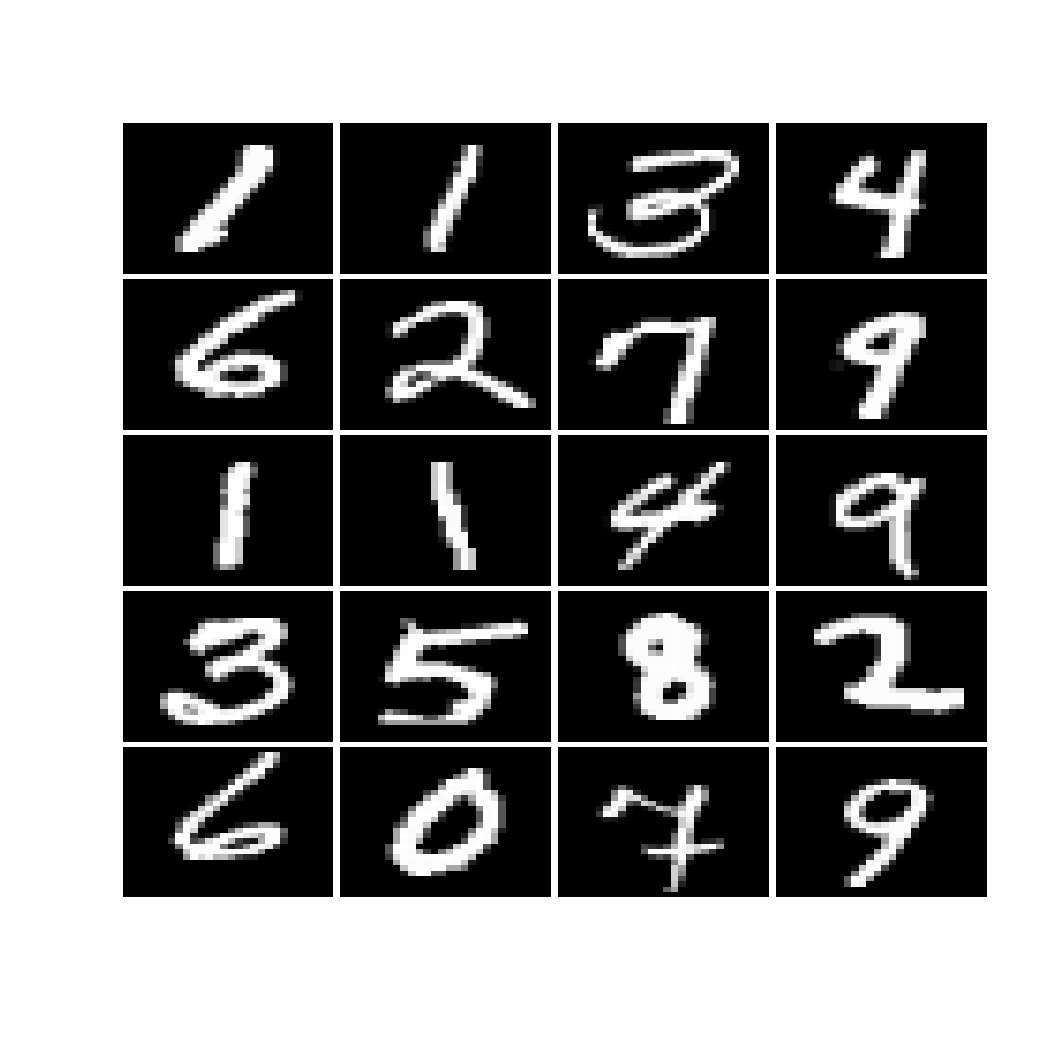
\includegraphics[scale=0.4]{digits}
	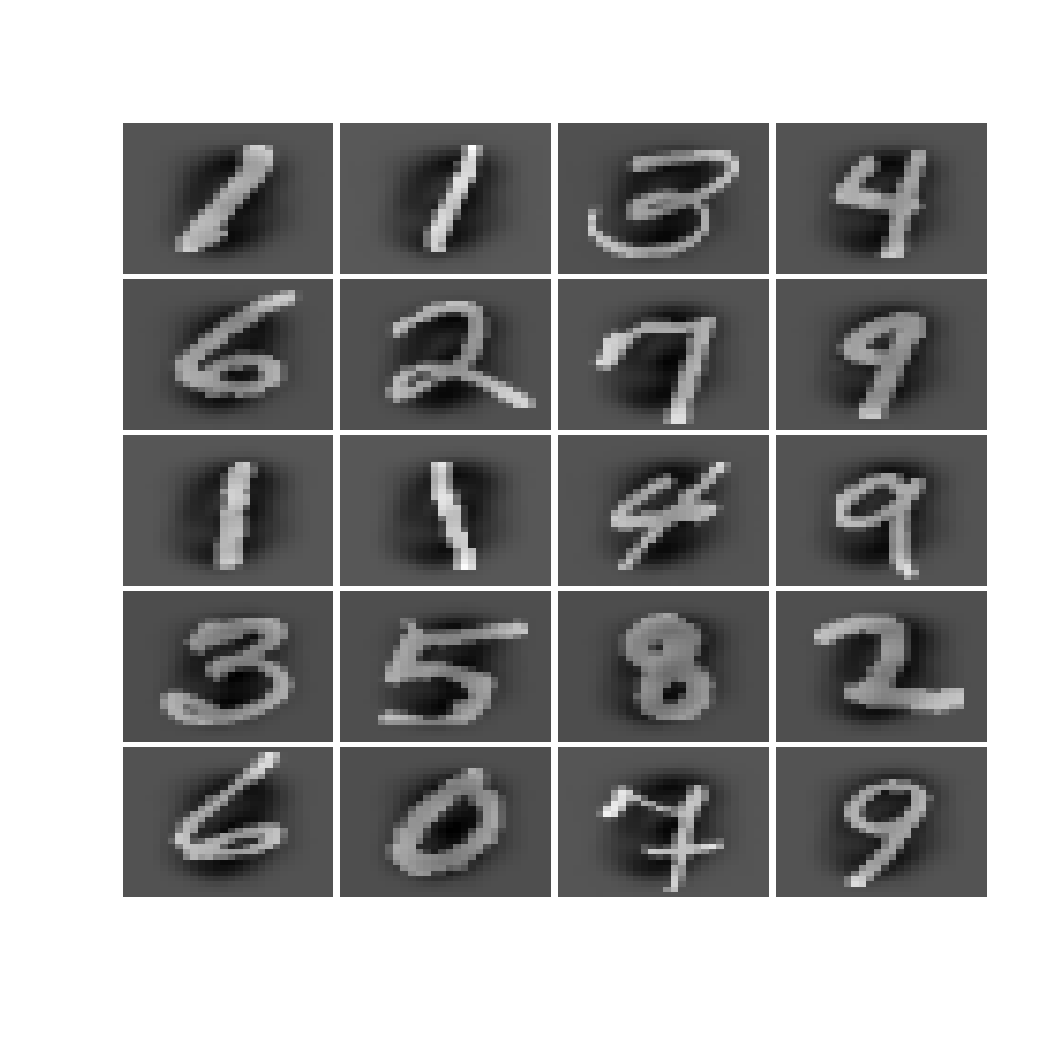
\includegraphics[scale=0.4]{digitspre}
	\caption{Visualization of the first 20 digits of the data before and after preprocessing.
	The preprocessing centerss and normalizes each digit and centers each variable.}\label{fig:digits}
\end{figure}

\subsection{Exercise 2}
The variances of the digit data explained by the number of principal components are displayed in Figure~\ref{fig:pcavar}.
The same figure displays visualizations of the actual principal components.
Because the principal components are vectors of the same length as each digit vector, they can be visualized the samy way as the digits.
As can be expected, the visualization shows that the principal components have non-zero values mostly near the center of the images, where the digits differ a lot from each other.
\begin{figure}\centering
	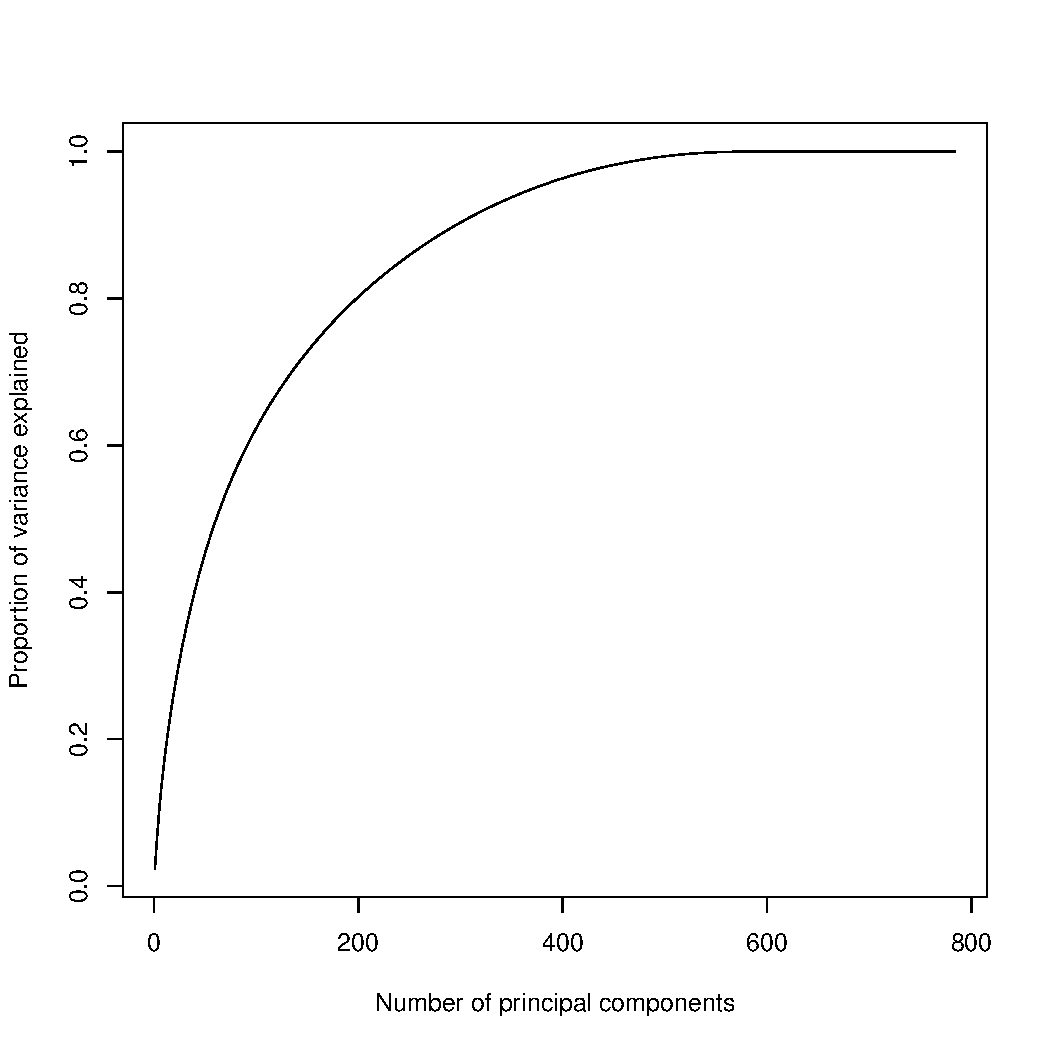
\includegraphics[scale=0.6]{pcavar}
	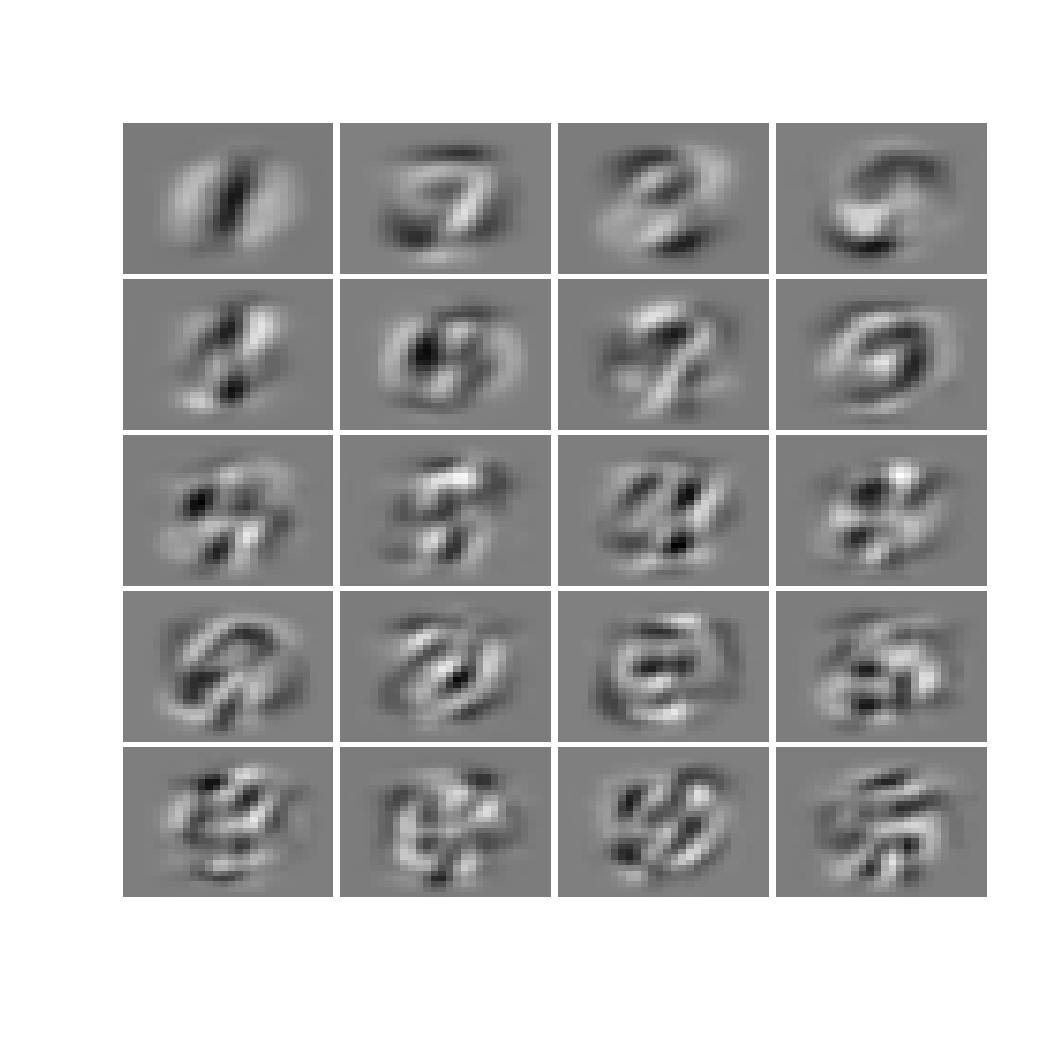
\includegraphics[scale=0.4]{pcanums}
	\caption{Left: the proportion of variance explained by the number of principal components.
	Right: visualization of the principal components.
The colors are scaled such that black and white parts of the images represend negative and positive valus in the PCs while grey pixels represent zero-values.}\label{fig:pcavar}
\end{figure}

\subsection{Exercise 3}
Let $Y$ be the $784\times 1000$ matrix obtained from the original matrix $X$ by preprocessing it as described in Section~\ref{sec:31}.
Denote by $P$ the $784\times 784$ matrix containing the principal components of $Y$ as its columns, and by $P^i$ its first $i$ columns.
We can reduce the dimension of $Y$ by multiplying it with $P$: $R^i=Y^TP^i$.
We can then reproduce an approximation to the original matrix by multiplying again by the transpose of $P^i$: $$(Y^i)^T=R^i(P^i)^T=Y^TP^i(P^i)^T.$$
The reconstruction error of a data vector is defined as the squared distance to the original data. The average error is the average of the errors of all the considered data vectors:
$$Err_i = \frac{1}{n}\sum_{j=1}^{n}||Y_{*j}-Y^i_{*j}||^2$$ where $Y_{*j}$ denotes the $j$th column of $Y$. The principal components minimize the reconstruction error of this dimension reduction.

The average reconstruction errors for different numbers of different numbers of principal components are displayed in Figure~\ref{fig:avgerr}.
It can be seen that the error goes down quickly during about the first 20 components but the differences become smaller after that.

Figure~\ref{fig:reduce} displays the result of doing dimension reduction and reconstruction for the 10 first digits using different numbers of principal components.
All the digits remain readable after reducing them to 16 first principal components.
With much fewer components, it becomes impossible to distinguish eg. 4 and 9 from each other.

The dimension reduction performed by projection to the principal component directions is also a form of lossy compression, because it represents approximately the same images using a smaller amount of values.
The method does not always reduce the total data size, as we need to store the first principal components to reproduce the data.
The size of the PCA matrix doesn't depend on the number of data vectors, only on the number of variables, so we can save space if we have a very large amount of similarly distributed data.
The data vectors should follow a similar distribution so that all of them can be recreated accurately using the same principal components.

\begin{figure}\centering
	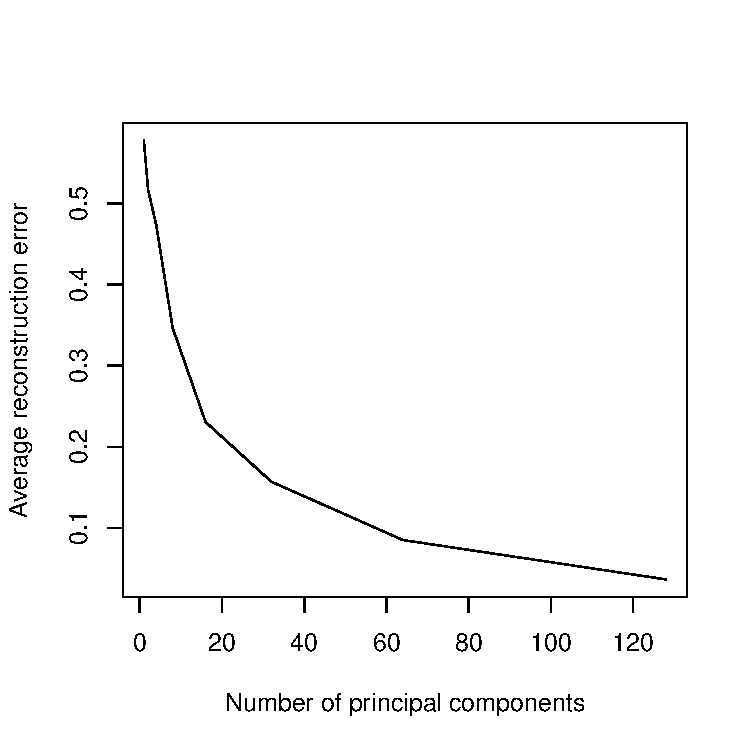
\includegraphics[scale=0.5]{error}
	\caption{The average reconstruction error of dimension reduction as a function of the number of principal components.}\label{fig:avgerr}
\end{figure}
\begin{figure}\centering
	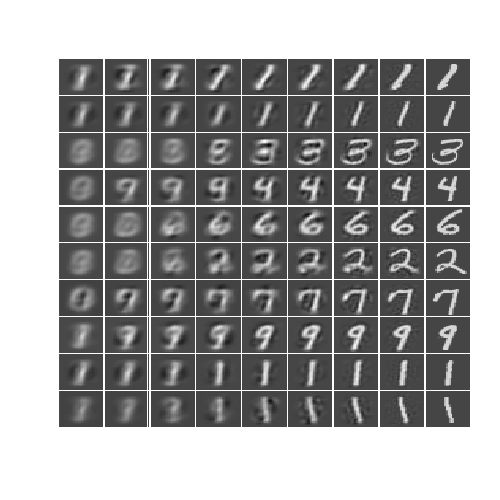
\includegraphics[scale=\sscale]{digitreduce}
	\caption{The first 10 digits after reducing them to 1, 2, 4, 8, 16, 32, 64 and 128 dimensional subspaces spanned by the first principal components.
The rightmost column contains the original digits.
The digits where preprocessed before the reduction and the preprocessing steps where inversed after the reduction.}\label{fig:reduce}
\end{figure}

\subsection{Exercise 4}

The dimension reduction with PCA can be used as a denoising method.
As we saw, digit images can be represented by a small number of principal component directions, so we can ignore all the variance in other directions as noise.
Since we use only a small number of principal components, the subspace spanned by their directions is only a small fraction of the whole space, so we ignore a large amount of the noise.
Note that the principal components we use are the principal components of the non-noisy digit images, because we don't want the components to represent the noise but the actual signal parts of the data.

Figure~\ref{fig:denoise} displays the result of denoising the noisy images by projecting them to some of the first principal components. It can be seen that many images are much more readable than the original ones when reduction is done with 16 components. With 8 components some digits become even clearer, but many also become too blurry to recognize. With 32 components most digits are quite hard to read, as much of the noise still remains.

\begin{figure}\centering
\newcommand{\dns}{0.45}
\subfigure[Original data]{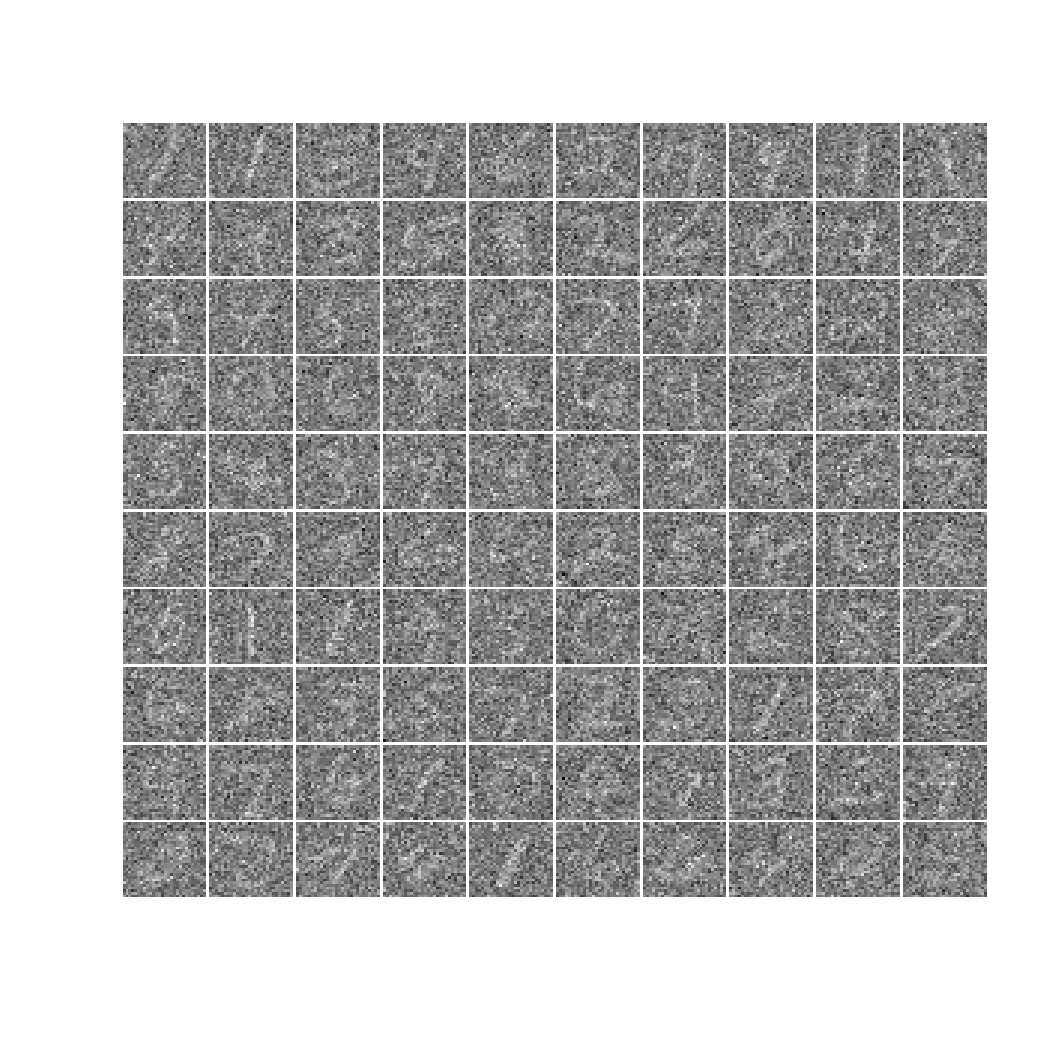
\includegraphics[scale=\dns]{noisy}\label{dno}}
\subfigure[Reduction using 8 components]{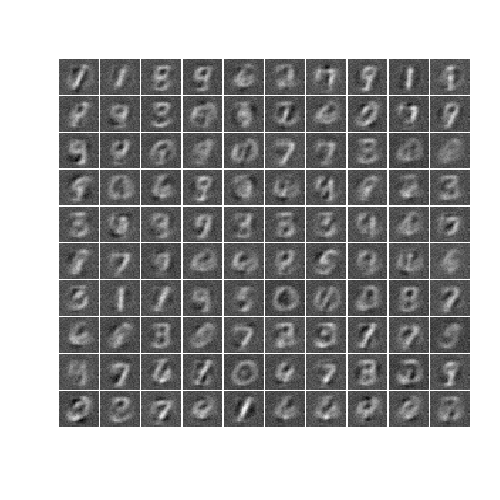
\includegraphics[scale=\dns]{denoise8}\label{dn8}}
\subfigure[Reduction using 16 components]{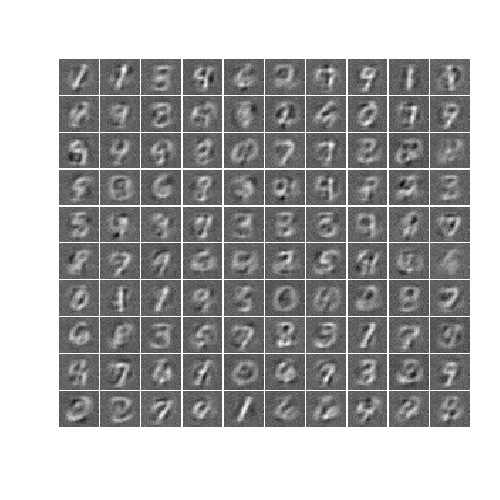
\includegraphics[scale=\dns]{denoise16}\label{dn16}}
\subfigure[Reduction using 32 components]{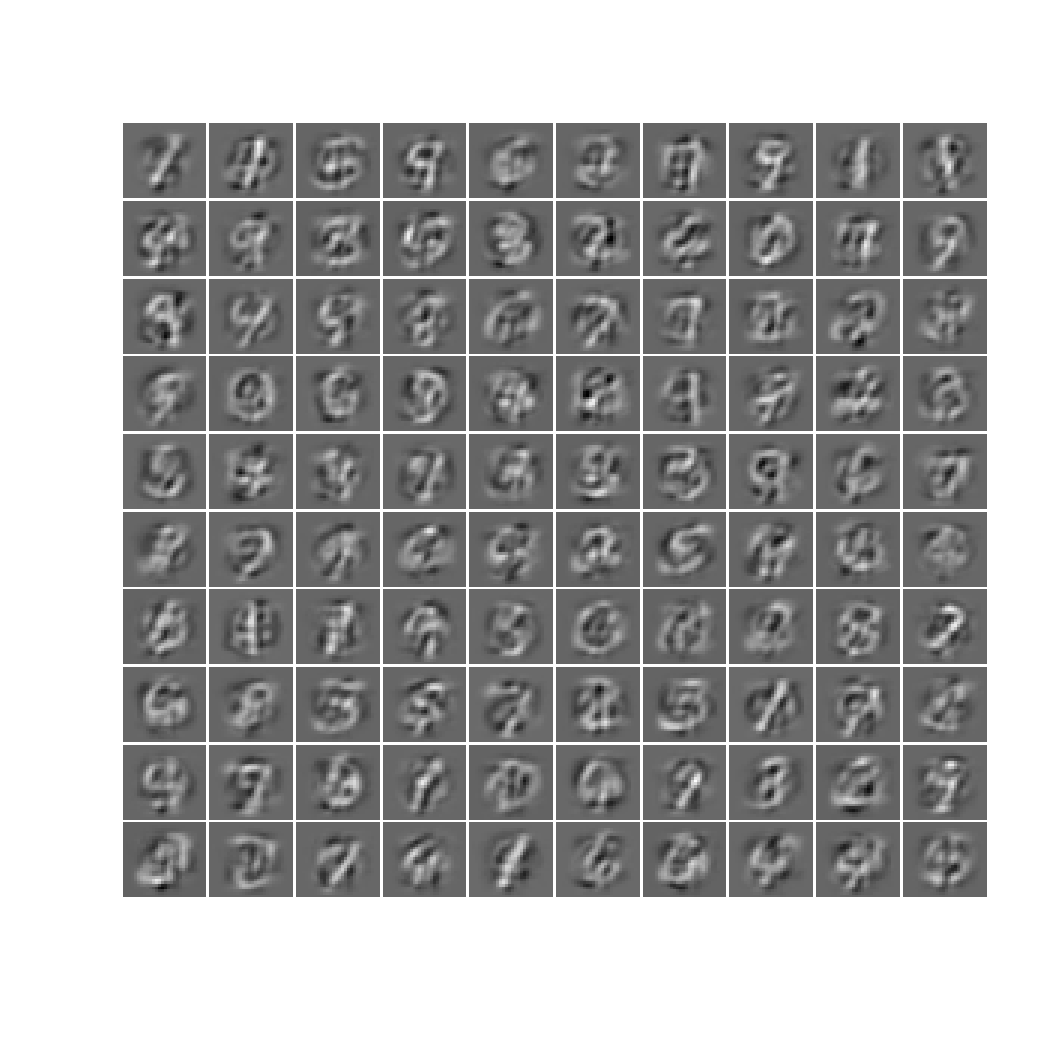
\includegraphics[scale=\dns]{denoise32}\label{dn32}}
%	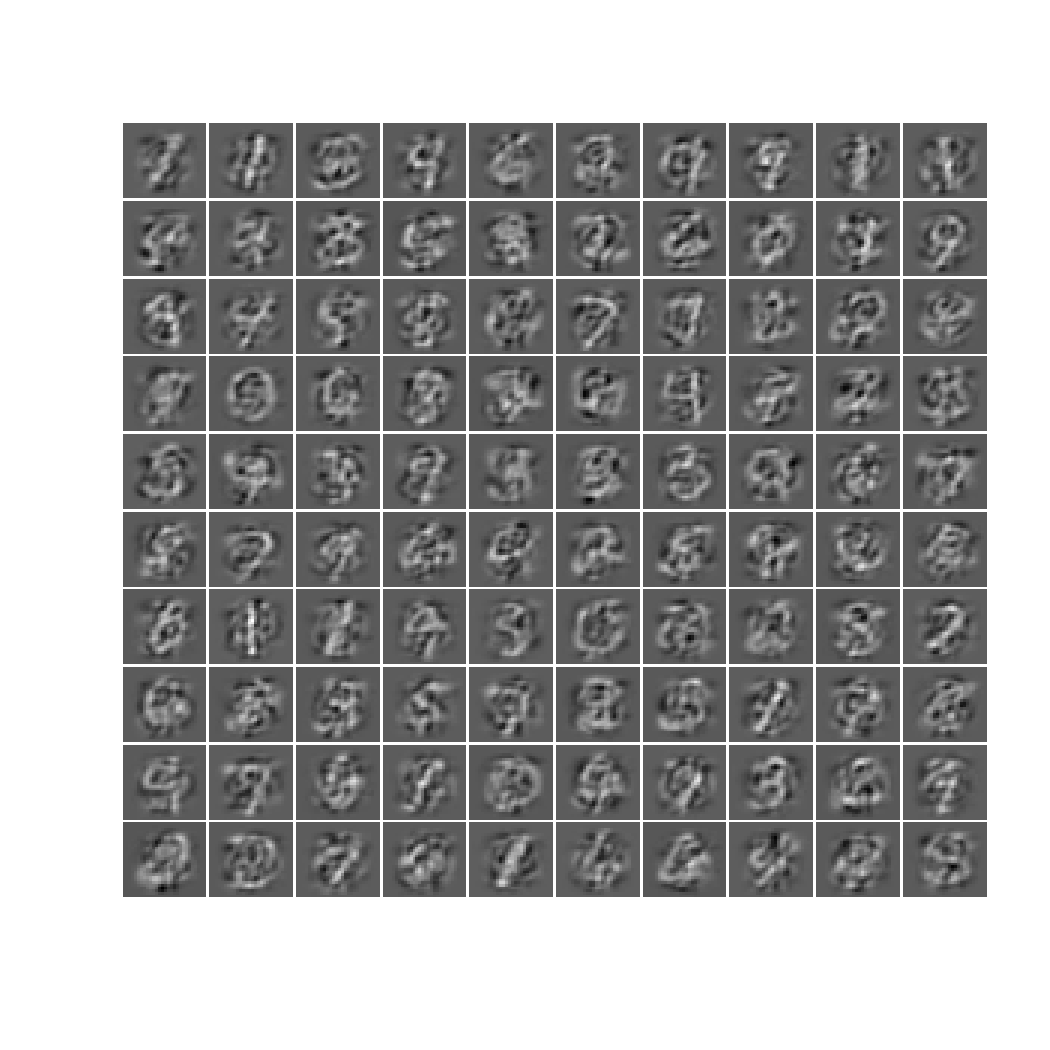
\includegraphics[scale=\dns]{denoise64}
\caption{The result of denoising noisy digit images using dimension reduction. The images are denoised by projecting them to low-dimensional subspace spanned by the first principal components of non-noisy digit images. The image~\ref{dno} contains the original images and the images~\ref{dn8},\ref{dn16},\ref{dn32} display the result of reduction to 8, 16 and~32 components respectively.}\label{fig:denoise}
\end{figure}

\end{document}
